%<dscrpt>Carrés, armures et satins.</dscrpt>
Ce problème porte sur les sommes de deux carrés de nombres entiers. On note
\begin{displaymath}
  \Sigma = \left\lbrace x^2 + y^2,\; (x,y)\in \Z^2\right\rbrace 
\end{displaymath}
On appelle \emph{entier de Gauss} un nombre complexe dont la partie réelle et la partie imaginaire sont des entiers relatifs. On  note $\Z[i]$ l'ensemble des entiers de Gauss.
\begin{displaymath}
  \Z[i] = \left\lbrace x +yi, (x,y)\in \Z^2\right\rbrace 
\end{displaymath}
\begin{figure}[h]
  \centering
  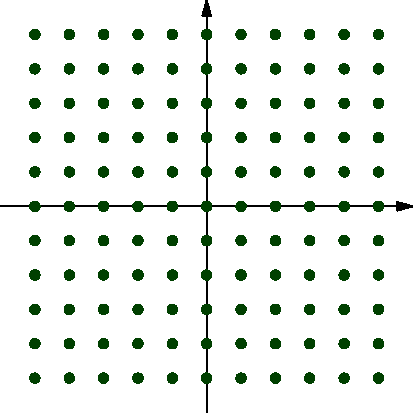
\includegraphics{./Eari2car_1.pdf}
  % Eari2car_1.pdf: 0x0 pixel, 0dpi, 0.00x0.00 cm, bb=
  \caption{Représentation des entiers de Gauss}
  \label{fig:Eari2car_1}
\end{figure}

\textbf{Question préliminaire.}\newline
Vérifier que $\Z[i]$ est un sous-anneau de $\C$ contenant $\Z$ c'est à dire que 
\begin{displaymath}
  \Z \subset \Z[i],\hspace{0.5cm} \forall(z,z')\in \Z[i]^2:\; z+z' \in \Z[i]\text{ et } zz'\in \Z[i]
\end{displaymath}
On introduit dans $\Z[i]$ des définitions arithmétiques analogues à celles de $\Z$; on convient de les noter en préfixant par un \og G-\fg.~ Par exemple:
\begin{itemize}
  \item Soit $u\neq 0$ et $v$ deux entiers de Gauss, on dit que $u$ \emph{G-divise} $v$ si et seulement si il existe $w\in \Z[i]$ tel que $v=uw$.
  \item Soit $u$ un entier de Gauss, on note $\Z[i]u$ l'ensemble des \emph{G-multiples} de $u$.
\begin{displaymath}
  \Z[i]u = \left\lbrace wu, w\in \Z[i] \right\rbrace 
\end{displaymath}  
\end{itemize}

\subsection*{Partie I. Arithmétique des entiers de Gauss.}
\begin{enumerate}
\item 
\begin{enumerate}
  \item Montrer que 
\begin{displaymath}
\forall z\in \Z[i],\; |z|^2 \in \N;\hspace{1cm}
\forall (z,z')\in \Z[i]^2,\;
|zz'|^2 = |z|^2\,|z'|^2
\end{displaymath}
  \item Montrer que, pour tout entier $n$,
\begin{displaymath}
  n\in \Sigma \Leftrightarrow \exists u\in \Z[i]\text{ tel que } n = |u|^2
\end{displaymath}
En déduire que le produit de deux éléments de $\Sigma$ est dans $\Sigma$.
  \item Soit $u\neq 0$ et $z$ dans $\Z[i]$. Montrer que si $u$ G-divise $z$ alors $|u|^2$ divise $|z|^2$. (divisibilité dans $\Z$)
\end{enumerate}

\item Un entier de Gauss $u$ est dit \emph{G-inversible} si et seulement si il existe $v\in \Z[i]$ tel que $uv=1$. 
\begin{enumerate}
  \item Montrer que $1$, $-1$, $i$, $-i$ sont G-inversibles, préciser les entiers de Gauss inverses.
  \item Soit $u$ un entier de Gauss G-inversible, montrer que $|u|^2=1$. En déduire l'ensemble des éléments G-inversibles.
\end{enumerate}

\item Un entier de Gauss non nul et non G-inversible $z$ est dit \emph{G-irréductible} si et seulement si, pour tout G-diviseur $v$ de $z$, $|v|=1$ ou $|v|=|z|$.
\begin{enumerate}
  \item \'Etudier le caractère G-irréductible de $1+i$, de $5$, d'un élément de $\Sigma$.
  \item Montrer que tout entier de Gauss non nul et non G-inversible est G-divisible par un entier de Gauss G-irréductible. En déduire qu'il est le produit d'un nombre fini de G-irréductibles.
\end{enumerate}

\item \emph{G-division euclidienne}.
\begin{enumerate}
  \item Montrer que, pour tout $x\in \R$, il existe $a\in \Z$ tel que $|x-a|\leq \frac{1}{2}$.
  \item Soit $u\neq 0$ et $z$ dans $\Z[i]$, montrer qu'il existe $q$ et $r$ dans $\Z[i]$ tels que 
\begin{displaymath}
  z = q u + r\text{ avec } |r|^2 < |u|^2
\end{displaymath}
(On pourra considérer le nombre complexe $\frac{z}{u}$.)
\end{enumerate}
\end{enumerate}


\subsection*{Partie II. Réseaux.}
Dans ce problème, un \emph{réseau} est une partie de $\Z[i]$ stable pour l'addition. Autrement dit, une partie $\mathcal{R}$ de $\Z[i]$ est un réseau si et seulement si
\begin{displaymath}
  \forall (z,z')\in \mathcal{R}^2,\; -z\in \mathcal{R} \text{ et } z+z' \in \mathcal{R}
\end{displaymath}
Il est évident que $\Z[i]$ est stable par conjugaison et multiplication par $i$. On définit les applications $c$, $s$ et $r$ de $\Z[i]$ dans $\Z[i]$ par:
\begin{displaymath}
  \forall z \in \Z[i],\; c(z) = \overline{z},\; s(z) = i\,\overline{z},\; r(z) = iz
\end{displaymath}
Un réseau $\mathcal{R}$ est dit 4-\emph{symétrique} si et seulement si il est stable par $r$ c'est à dire :
\begin{displaymath}
  \forall z\in \mathcal{R},\; r(z) = iz \in \mathcal{R}
\end{displaymath}
Soit $n\geq 2$ un entier naturel. On définit $\mathcal{S}_n$ et $\mathcal{T}_n$ par:
\begin{displaymath}
  \mathcal{S}_n = \left\lbrace z\in \Z[i] \text{ tq } \Re(z) \equiv \Im(z) \mod n\right\rbrace ,
\;
  \mathcal{T}_n = \left\lbrace z\in \Z[i] \text{ tq } \Im(z) \equiv 0 \mod n\right\rbrace 
\end{displaymath}

\begin{enumerate}
\item Vérifier que $s\circ c = -c\circ s = r$.

\item Soit $u\in \Z[i]$. Montrer que $\Z[i]u$ est un réseau et qu'il est 4-symétrique.\newline
Un réseau $\mathcal{R}$ est dit \emph{carré} si et seulement si il existe $u\in \Z[i]$ tel que $\mathcal{R} = \Z[i]u$. Comment peut-on justifier ce terme?  
  
\item Soit $n\geq 2$ un entier naturel. Montrer que $\mathcal{S}_n$ et  $\mathcal{T}_n$ sont des réseaux. Pour quelles valeurs de $n$ le réseau $\mathcal{S}_n$ est-il 4-symétrique?

\item On se propose de montrer que tout réseau 4-symétrique est carré.\newline
Soit $\mathcal{R}$ un réseau 4-symétrique non réduit à $0$.
\begin{enumerate}
  \item Soit $u \in \mathcal{R}$. Montrer que  tout G-multiple de $u$ est dans $\mathcal{R}$.

  \item Montrer qu'il existe $u_0\in \mathcal{R}$ non nul tel que 
\begin{displaymath}
\forall v \in \mathcal{R}, \;v\neq 0 \Rightarrow  |u_0|^2 \leq |v|^2 
\end{displaymath}
  \item Montrer que $\mathcal{R} = \Z[i]u_0$. Dans quel cas a-t-on $|u_0|=1$?
\end{enumerate}
\end{enumerate}

\subsection*{Partie III. Armures et satins.}
Dans cette partie \footnote{D'après \href{http://www.math.ens.fr/culturemath/histoire\%20des\%20maths/pdf/Decaillot\_textile.pdf}{La géométrie des tissus} d'\'Edouard Lucas. L'armure est le mode d'entrecroisement des fils de chaîne et des fils de trame. Les armures peuvent être représentées par des réseaux $\mathcal{R}_a$.}, $p$ désigne un nombre premier et $a\in \Z$. On définit $\mathcal{R}_a$ par
\begin{displaymath}
\mathcal{R}_a = \left\lbrace  xp + yip + z(1+ia), (x,y,z)\in \Z^3 \right\rbrace  
\end{displaymath}
\begin{figure}[h]
  \centering
  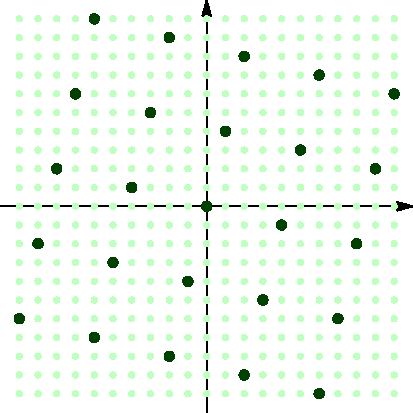
\includegraphics{./Eari2car_2.pdf}
  \caption{Un réseau carré.}
  \label{fig:Eari2car_2}
\end{figure}

\begin{enumerate}
  \item 
\begin{enumerate}
  \item Montrer que $\mathcal{R}_a$ est un réseau.
  \item Montrer\footnote{Notations $\mathcal{T}$ pour \emph{toile} et $\mathcal{S}$ pour \emph{sergé} : des types particuliers de tissus.} que $\mathcal{R}_0 = \mathcal{T}_p$ et que $\mathcal{R}_1 = \mathcal{S}_p$.
  \item Soit $a$ et $b$ dans $\Z$, montrer que
\begin{displaymath}
  \mathcal{R}_a = \mathcal{R}_b \Leftrightarrow a \equiv b \mod p  
\end{displaymath}
\end{enumerate}

\item On suppose que $a\not \equiv 0 \mod p$. On dit dans ce cas que $\mathcal{R}_a$ est un \emph{satin}.
\begin{enumerate}
  \item Montrer qu'il existe $a'\in \Z$ tel que $aa' \equiv 1 \mod p$.
  \item Montrer que $c(\mathcal{R}_a) = \mathcal{R}_{-a}$ et que $s(\mathcal{R}_a) = \mathcal{R}_{a'}$.
  \item Montrer que si $a'\equiv -a \mod p$ alors $\mathcal{R}_a$ est carré.
  \item Le réseau de la figure \ref{fig:Eari2car_2} est un satin. Déterminer $p$ et $a$ et vérifier qu'il est bien carré.
\end{enumerate}
\item
\begin{enumerate}
  \item Montrer que 
\begin{displaymath}
\forall (z,z')\in \Z[i]^2,\;
\Im(\overline{z}z') \in \Z
\end{displaymath}

  \item Montrer que
\begin{displaymath}
  \forall (u,u')\in \mathcal{R}_a^2,\; \Im(\overline{u}\,u') \equiv 0 \mod p
\end{displaymath}
En déduire que $\mathcal{R}_a \neq \Z[i]$.
  \item Montrer que, dans un satin $\mathcal{R}_a$, il existe $u$ et $u'$ tels que $\Im(\overline{u}\,u') =p$.  
\end{enumerate}


\item On suppose qu'il existe $a\in \Z$ tel que $a^2 + 1 \equiv 0 \mod p$.
\begin{enumerate}
  \item Montrer que $\mathcal{R}_a$ est carré.
  \item Montrer que $p$ est la somme de deux carrés d'entiers. 
\end{enumerate}

\end{enumerate}

\subsection*{Partie IV. Sommes de deux carrés.}
Notons $\mathcal{P}_c$ l'ensemble des nombres premiers $p$ pour lesquels $-1$ est un carré modulo $p$ c'est à dire tels que 
\begin{displaymath}
  \exists a\in \Z \text{ tel que } a^2 + 1 \equiv 0 \mod p
\end{displaymath}
Notons $\mathcal{P}_c'$ l'ensemble des nombres premiers qui ne vérifient pas cette propriété. On forme ainsi une partition de l'ensemble $\mathcal{P}$ de tous les nombres premiers.
\begin{enumerate}	
  \item
\begin{enumerate}
  \item Montrer que $\mathcal{P}_c \subset \Sigma$.
  \item Soit $n$ entier naturel non nul. On considère sa décomposition en facteurs premiers. Montrer que si les valuations $v_p(n)$ sont paires pour les diviseurs premiers dans $\mathcal{P}_c'$, alors $n\in \Sigma$.
\end{enumerate}
\item Soit $p$ un nombre premier dans $\Sigma$ avec $p=x^2+y^2$ pour $x$ et $y$ non nuls dans $\Z$.
\begin{enumerate}
  \item Montrer qu'il existe $\lambda$ et $\mu$ dans $\Z$ tels que $\lambda x - \mu y = 1$. On pose $a = \lambda y + \mu x$.
  \item Exprimer $x$ et $y$ en fonction de $\lambda$, $\mu$, $a$.
  \item Montrer que $(\lambda^2 + \mu^2)p = 1 +a^2$. En déduire que $p\in \mathcal{P}_c$.
\end{enumerate}

\item Montrer que tout $p \in \mathcal{P}_c'$ est G-irréductible. En déduire, pour tout nombre premier $p$, l'équivalence entre les trois propositions.
\begin{displaymath}
  p\in \Sigma \Leftrightarrow p\in \mathcal{P}_c \Leftrightarrow p \text{ n'est pas G-irréductible}
\end{displaymath}

\item
\begin{enumerate}
  \item Présenter un G-algorithme d'Euclide et justifier sa terminaison.
  \item Définir une notion de G-pgcd et énoncer un G-théorème de Bezout.
  \item Calculer un G-pgcd de $5+5i$ et de $-3+4i$.
\end{enumerate}

\item 
\begin{enumerate}
  \item \'Enoncer et démontrer un G-théorème de Gauss.
  \item Soit $n\in \Sigma$ et $p \in \mathcal{P}_c'$ un diviseur premier de $n$. Montrer $p^2$ divise $n$ et que le quotient est dans $\Sigma$. En déduire que la valuation $v_p(n)$ est paire.
\end{enumerate}

\end{enumerate}

\subsection*{Partie V. Congruences modulo 4.}
Cette partie utilise la définition de $\mathcal{P}_c$ de la partie IV mais aucun des résultats démontrés dans les parties précédentes.\newline
Soit $p>2$ un nombre premier et $I=\llbracket 1, p-1 \rrbracket$.
\begin{enumerate}
  \item Soit $x\in I$.  Préciser l'unique élément de $I$ congru à $-x$ modulo $p$. Montrer qu'il existe dans $I$ un unique élément noté $x'$ tel que $xx'\equiv 1 \mod p$. Cette notation $x'$ est valable dans toute la partie.
  \item On définit dans $I$ une relation $\bowtie$ par:
\begin{displaymath}
  \forall (x,y)\in I^2,\; x \bowtie y \Leftrightarrow (x^4+1)y^2 \equiv (y^4+1)x^2 \mod p
\end{displaymath}
Montrer que $\bowtie$ est une relation d'équivalence.
\item 
\begin{enumerate}
  \item L'équation $x \equiv -x \mod p$ admet-elle une solution dans $I$?
  \item Déterminer les $x\in I$ tels que $x=x'$.
  \item On considère l'équation $x=p-x'$ avec $x\in I$. Déterminer l'ensemble des solutions dans le cas où il existe $a\in I$ tel que $a^2+1\equiv 0 \mod p$.\newline
  Que se passe-t-il lorsqu'il n'existe pas un tel $a$?
\end{enumerate}
\item Factoriser 
\begin{displaymath}
  (x^4+1)y^2 - (y^4+1)x^2
\end{displaymath}
En déduire la classe d'équivalence pour $\bowtie$ d'un $x\in I$.

\item Montrer que $p\in \mathcal{P}_c$ si et seulement si $p\equiv 1 \mod 4$.
\end{enumerate}

